%% This is an example first chapter.  You should put chapter/appendix that you
%% write into a separate file, and add a line \include{yourfilename} to
%% main.tex, where `yourfilename.tex' is the name of the chapter/appendix file.
%% You can process specific files by typing their names in at the 
%% \files=
%% prompt when you run the file main.tex through LaTeX.
\chapter{Motivación del diseño y desarrollo de XRemotebot}\label{ch1}
% FIXME \section{Motivación del diseño y desarrollo de XRemotebot}\label{ch1:motivacion}

Desde el año 2009, en el marco del proyecto ``Programando con robots y
software libre'' de la Facultad de Informática,
se brindan cursos de programación en Python para alumnos de escuelas
secundarias utilizando robots didácticos.

En un comienzo se utilizaron los robots Scribbler de Parallax
(figura~\ref{fig:robots_usados_scribbler}), los mismos se
pueden programar directamente a través de un cable en el lenguaje
PBASIC y funcionar de forma autónoma o pueden ser controlados de forma
inalámbrica con Bluetooth, durante las actividades se utilizó de la última
forma que permite controlarlo usando el lenguaje Python cuyo intérprete no
es posible ejecutar directamente sobre el microcontrolador del robot.

Estos robots se importaban desde Estados Unidos en volúmenes bajos lo que
dificultaba su adquisición y dejaba al equipo sin ninguna garantía ante
averías, por estos motivos se buscaron alternativas de fabricación nacional,
que pudieran utilizarse desde Python y tuvieran especificaciones abiertas.
De esta manera en el año 2011 se adquirieron para pruebas robots Multiplo N6
de la empresa RobotGroup (figura~\ref{fig:robots_usados_n6})
cuyas especificaciones se distribuyen bajo una licencia libre y
la empresa se comprometió a la creación de una biblioteca Python que permitiera
su programación en ese lenguaje, esa biblioteca se desarrolló en conjunto
con miembros del laboratorio LINTI y miembros de la empresa RobotGroup siendo
mantenida en la actualidad por los primeros. Los robots Multiplo N6 son
controlados por una placa basada en Arduino, la misma se puede programar
a través de un cable en el lenguaje C++ de manera que el robot luego funcione
de manera autónoma y también pueden ser controlados de forma inalámbrica
a través del protocolo ZigBee~\citep{diaz_aprendiendo_2012}. La placa
controladora del N6 se denomina DuinoBot y no debe confundirse con la biblioteca
Python del mismo nombre que se desarrolló en conjunto con la empresa RobotGroup
para controlar estos robots. De aquí en adelante se denominará DuinoBot a la
biblioteca y placa controladora al componente de hardware que contiene el
microcontrolador a menos que se especifique lo contrario.



En el año 2012, a través de una cooperación con la Fundación YPF que brindó
un subsidio y bajo el auspicio de la Dirección de Escuelas Técnicas de la
Provincia de Buenos Aires se dictaron cursos en 10 escuelas técnicas de la
provincia. La fundación YPF brindó a cada una de estas escuelas, entre otras
cosas, 20 robots Multiplo N6 que quedarían en cada escuela, en estos cursos
se capacitó a 140 docentes y 40 alumnos avanzados en programación en Python
a través del uso de estos dispositivos~\citep{diaz_aprendiendo_2012}.
Esta experiencia consolidó el uso de
los robots N6 para los cursos dictados en el marco del proyecto
``Programando con robots y software libre'' donde estos robots desplazaron
a los Scribblers por su confiabilidad y stock, dadas las dificultades de
reponer los Scribblers a medida que se averiaban por los motivos
ya mencionados.

\begin{figure}
    \centering
    \begin{subfigure}[b]{0.49\textwidth}
        \includegraphics[width=\textwidth]{figures/scribbler}
        \subcaption{Robot Scribbler de Parallax}
        \label{fig:robots_usados_scribbler}
    \end{subfigure}
    \begin{subfigure}[b]{0.49\textwidth}
        \includegraphics[width=\textwidth]{figures/n6}
        \subcaption{Robot Multiplo N6 de RobotGroup}
        \label{fig:robots_usados_n6}
    \end{subfigure}
    \caption{Robots usados en el proyecto}
    \label{fig:robots_usados}
\end{figure}

Aunque se han utilizado a la fecha estos dos modelos distintos de robots,
en esencia, las características principales de ambos modelos son las mismas
y coinciden con las de otros robots usados en la Argentina para enseñar a
programar, a saber:
\begin{itemize}
    \item El medio de locomoción es con 2 motores continuos que mueven cada
        uno una de las ruedas laterales.
    \item Cuentan con algún sensor o sensores que permiten detectar obstáculos.
    \item Cuentan con algún sensor o sensores que permiten detectar líneas.
    \item Operan sin el uso de cables
\end{itemize}

Cabe destacar sobre este último ítem que algunos de los robots no requieren
cables para operar ya que son programados con anterioridad a través de un
cable (usualmente USB o Serial) normalmente en algún lenguaje como C, Assembler
o Basic. Pero los robots usados en el proyecto antes mencionado no requieren cables ya que son controlados a través de señales
inalámbricas lo que permite controlarlos en tiempo real y utilizando
un intérprete Python estándar (cPython) instalado en el dispositivo
controlante.

Dado el costo y fragilidad de los robots habitualmente los alumnos interactúan
con los mismos solamente en el aula, ya sea en su escuela si la misma pudo adquirir los mismos o en las instalaciones de la  Facultad de Informática si el alumno
realiza alguna pasantía o práctica en la misma. Esto tiene varias connotaciones:
\begin{itemize}
    \item El alumno al estar en una situación formal en la escuela
        compartiendo el recurso limitado que es el robot con otros
        alumnos posiblemente no tenga el tiempo o el ambiente más apropiado
        para experimentar de forma lúdica con el robot.
    \item La tarea para casa solamente es realizable a través de un simulador
        que puede ser lo suficientemente completo y fiel como para aprender
        a programar, pero resulta menos estimulante y realista que manipular
        un robot real.
    \item Alumnos de escuelas que no tienen los recursos necesarios para
        adquirir el equipamiento o de escuelas alejadas de La Plata que
        no tienen la posibilidad de acercarse a nuestra
        Facultad no pueden interactuar con robots reales
        (a lo sumo podrán usar un simulador).
\end{itemize}

Por otro lado los dongles XBee que permiten conectarse con los robots
Multiplo N6
son relativamente costosos, el esquema normal de conexionado entre dispositivos
controladores y robots descripto en el capítulo~\ref{cha:arquitectura} requiere
2 dongles XBee por robot, uno conectado directamente al robot y el otro
conectado por USB al dispositivo controlante. En consecuencia:
\begin{itemize}
    \item El dispositivo controlante debe tener un puerto USB y los drivers
        necesarios para detectar la interfaz serial con el XBee, esto deja
        fuera de juego celulares y tablets.
    \item El costo de operar cada robot en este esquema es sensiblemente
        superior al costo que tendría si varios alumnos pudieran
        controlar varios robots usando un solo dispositivo XBee compartido
        entre varios dispositivos controlantes.
\end{itemize}

Tomando estos dos grupos de problemáticas se propone implementar una solución
que permita
superarlos de forma simultánea, esta solución permite controlar los
robots a través de una red, como puede ser Internet, permitiendo a los alumnos
conectarse a los robots desde sus hogares y a las instituciones a compartir
el uso de sus robots. Por otro lado también es posible configurar el servidor
para su uso en el aula deshabilitando funcionalidades innecesarias en un ámbito
local como ser la necesidad de autenticar a los usuarios para utilizar los
robots, este modo de operación fue pensado para que múltiples alumnos puedan
acceder a múltiples robots contando con un solo adaptador USB a XBee, esto
reduciría sensiblemente el costo de cada robot por alumno ya que de otra
manera por cada robot deberían usarse 2 dispositivos XBee (uno en el robot
y otro en la computadora del alumno) reduciéndose con este modo de operación
a un XBee por robot más un único adaptador USB a XBee conectado al servidor.

Como consecuencia de estos requerimientos quedaba claro que el servidor
debía tener una interfaz web y proveer acceso concurrente con relativa
baja latencia para permitir a múltiples alumnos acceder a múltiples robots
al mismo tiempo. Tener un servidor web basado en protocolos estándar hizo
que el requerimiento de que el cliente estuviera escrito en Python fuera
artificial dado que sería posible implementar clientes en cualquier lenguaje
que soporte estos protocolos. Esto dio lugar a la posibilidad de
implementar otros clientes que permitieran usar los robots en cursos
de programación de distintos lenguajes sin reimplementar el protocolo
de bajo nivel lo que hace en opinión del autor más sencilla la creación
de nuevos clientes en distintos lenguajes.
En especial la elección de protocolos y tecnologías usadas
y la falta de necesidad de acceder directamente al hardware a través de USB
habilita la implementación de un cliente Javascript que se ejecute en el
navegador Web de los usuarios.

El nivel de abstracción que puede proveer esta API hace que también sea
natural pensar en la posibilidad de manejar distintos tipos de robots
que tengan algunas características mínimas en común con los robots ya
descriptos.

El servidor Remotebot original (figura~\ref{fig:arquitectura_remotebot})
tenía algunas de estas características, pero
estaba pobremente implementado ya que no era más que una herramienta auxiliar
para un cliente muy específico y era meramente un intermediario entre el
cliente original implementado en Java y el módulo DuinoBot. Este servidor
estaba severamente limitado
ya que no era configurable, no contaba con ninguna forma de visualizar a los
robots de forma remota, no permitía autenticación, no disponía un sistema
de reserva de robots por lo que un cliente podía interferir en la operación
de un robot de otro cliente y las operaciones bloqueantes de un cliente
impedían el uso de los robots al resto de los clientes hasta que esa operación
terminase.

% FIXME: CREO QUE ESTARÍA BUENO QUE ACA PONGAS UNA FIGURA CON LA ARQUITETURA DE REMOTEBOOT
% Lo puse en otra sección donde se habla más en detalle. Fernando. Armé otra
% que muestra como se conectan, tengo límite poco claro entre lo que le digo
% arquitectura y los diagramas de bloque...

\begin{figure}
    \centering
    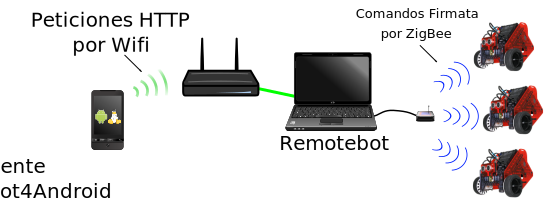
\includegraphics[width=\textwidth]{figures/arquitectura_remotebot}
    \caption{Esquema de conexión de Remotebot}
    \label{fig:arquitectura_remotebot}
\end{figure}


\section{Alternativas similares a XRemotebot}

Existen diferentes alternativas para controlar robots o microcontroladores
de forma remota, muchas de estas se agrupan bajo la denominación
``Internet of Things'', en este capítulo se describirán algunas de las
más destacadas y las más similares a XRemotebot.

% FIXME: mmmm NO SE SI ESTO DEBERÍA ESTAR EN UN CAPITULO APARTE.....  LO HABLAMOS LUEGO

\subsection{Educabot}
%~\citep{_educabot_2015}[REF]%
El proyecto Educabot~\footnote{\url{http://www.educabot.org/}} tiene por
objetivos enseñar tecnología a niños y adultos a través
del uso, programación y construcción de robots. En el sitio del proyecto
se ofertan cursos orientados a los distintos niveles.

% FIXME: ES ORIGINARIO DE ..... EN ESCUELAS? EN ONGS? DONDE SE LOS USA?

En la parte de construcción este proyecto plantea un modelo de robot denominado
``Rolo'' para los jóvenes de más de 10 años, mientras que para los más chicos
se plantean actividades con el robot ``elBrian'' que incluyen
controlarlo a través de una interfaz Web que muestra las imágenes emitidas
por la cámara incorporada en este robot y además permite controlarlo con
botones en pantalla que determinan en qué dirección debe moverse el robot
(figura~\ref{fig:elbrian}).

\begin{figure}
    \centering
    \includegraphics[width=0.5\textwidth]{figures/elbrian-1}
    \caption{Pantalla principal de elBrian (en el recuadro rojo normalmente
        se muestra la cámara de el robot)}
    \label{fig:elbrian}
\end{figure}

Las tecnologías utilizadas en la interfaz web de ``elBrian'' coinciden en gran
parte con las utilizadas en el desarrollo de XRemotebot, pero el objetivo del
servidor CUAL???? es controlar un único robot en un ambiente local y además este servidor
se instala en el robot cuestión que sería imposible en los robots basados en
microcontroladores AVR y Parallax (ojo!!!!  ESTO NOMBRALO ANTES PLEASE!!! ) a los que XRemotebot se encuentra dirigido.


El servidor web de ``elBrian'' está implementado usando el framework Tornado,
Websockets, mjpg-streamer, opencv y JSON. El mismo está diseñado para ejecutarse
en el robot ya que el mismo está basado en una placa RaspberryPi, la cuál
cuenta con un procesador ARM perfectamente capaz de ejecutar un sistema
operativo completo como GNU/Linux y de soportar el intérprete oficial de Python.

Mientras que este servidor coincide en gran medida en la elección de lenguaje
y bibliotecas utilizadas su implementación es específica para el robot ``elBrian''
y no podría ser portada para robots con menores capacidades de procesamiento
sin una reescritura significativa. Además el protocolo utilizado no contempla
el acceso a valores de sensores, los únicos mensajes que permite enviar
al robot son movimientos.

\begin{itemize}
    \item Educabot \url{http://www.educabot.org/}
    \item Código fuente de ``elBrian'' \url{https://github.com/educabot/elBraian}
\end{itemize}

\subsection{Gobot con cppp-io}

Gobot {REF} es una biblioteca que permite controlar robots programando en el lenguaje
Go[REF], esta biblioteca soporta el protocolo Firmata (IDEM CON ESTAS COSAS.... ACLARA, PONE REFERENCIAS O NOMBRLAS ANETES) para controlar robots
conectados directamente a través de una interfaz serial, como es el caso
de los robots Multiplo N6, y soporta la API cppp-io{REF] que define una API JSON
que permite el acceso a la información y control de robots a través de la Web.

Gobot además tiene compatibilidad con distintos sensores y robots, además de
placas utilizadas normalmente en la construcción de robots como Arduino,
Raspberry Pi, Intel Edison y Beaglebone Black.

Este proyecto es interesante como base para desarrollar algún proyecto
similar a XRemotebot en Go, pero requeriría además la reimplementación
del módulo de Python DuinoBot que controla, a través de una versión
modificada del protocolo Firmata, a los robots Multiplo N6 y por otro
lado los robots Scribbler tampoco aparecen en la lista de robots soportados.

\begin{itemize}
    \item Gobot \url{http://gobot.io}
    \item Especificación de cppp-io \url{https://github.com/hybridgroup/cppp-io/}
\end{itemize}

\subsection{Tele Toyland}

Este sitio provee acceso a varios dispositivos a través de una interfaz web,
por ejemplo es posible controlar un cabezal con una punta que dibuja sobre
una caja de arena, basta con hacer clic sobre las posiciones sobre las cuales
se quiere que pase la punta y presionar el botón ``go'' para que el cabezal
empiece a moverse dibujando lo pedido, en este y el resto de los experimentos
disponibles en el sitio los resultados se pueden ver a través de un streaming
de video.

El sitio no provee detalles del software, ni el protocolo utilizado.

\begin{itemize}
    \item \url{http://www.teletoyland.com}
\end{itemize}

% FIXME
%\subsection{}
%http://www3.uji.es/~pnebot/Files/Articuls/RemoteProgramming.pdf
%Otro
%http://telerobot.mech.uwa.edu.au/Telerobot/instructions.html
\subsection{DIY}
% www.linuxuser.co.uk/tutorials/control-your-raspberry-pi-robot-from-a-web-connected-device
Finalmente en la consigna de ``do it yourself'' existen diversas guías para
programar servidores que permitan controlar robots o microcontroladores
en general, se puede encontrar un caso muy bien explicado en el sitio
de Adafruit~\url{https://learn.adafruit.com/wifi-controlled-mobile-robot/building-the-web-interface},
este es un buen ejercicio de programación, sobre todo para aprender a
programar servidores que provean una API web y clientes que la consuman. Sin
embargo estas guías son introductorias y el objetivo es crear un servidor
muy simple, similar a lo que fue el servidor Remotebot, pensados para ser
usados en un ambiente local ya que no proveen autenticación en general.

